\subsection{Error and convergence study}
\label{sec:analysis}

Figure~\ref{fig:rlzs} shows the evolution of the
water surface elevation for the 125 realizations obtained 
to compute the PC expansions at the four different gauge 
locations. We notice that the variation in surface elevation 
is negligible during the first hour at gauge number 21418 
and during the first two hours for the remaining gauges
as the plots of the different realizations are seen to superimpose.
However, a noticeable uncertainty in the surface 
elevation can be seen  at all gauges as indicated from the thickness 
of the bands formed by the plots of the realizations. This uncertainty
occurs till the end of the simulations.
\begin{figure}[h]
\centering
\begin{tabular}{clc}        
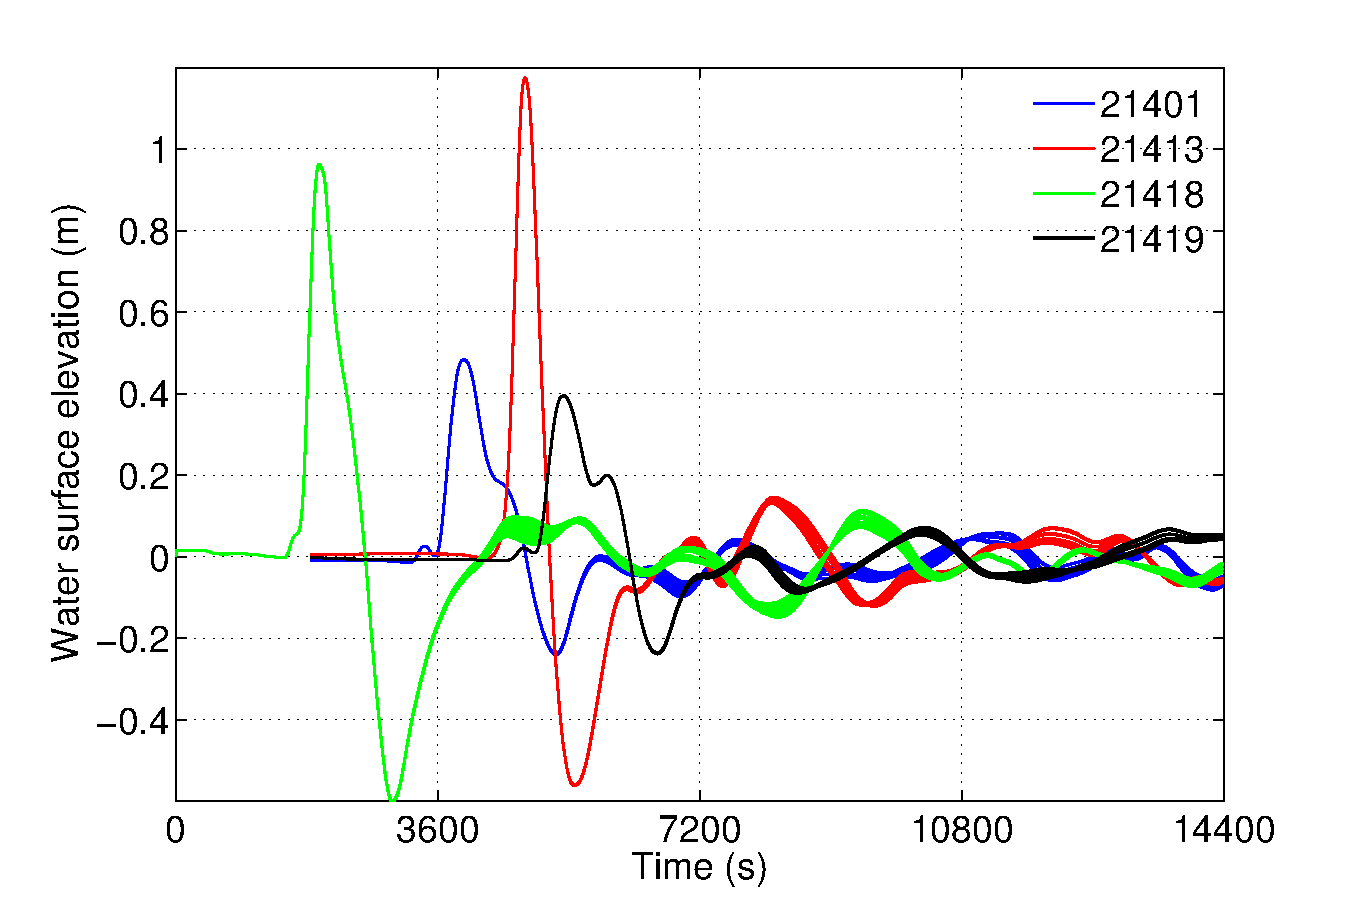
\includegraphics[width=0.6\textwidth]{../figures/rlzs_gauges.pdf} 
\end{tabular}
\caption{125 Geoclaw realizations at different gauge locations.}
\label{fig:rlzs}
\end{figure}


In order to check the consistency of the approximation, we compare
 water surface elevation from the realizations 
with those obtained from the PC surrogate. The different curves
show an excellent agreement (not shown) for all times. We also define
an error metric that measures the relative normalized root mean-square error between the left hand side function 
in Equation~(\ref{eq:stochseries})
and its PC representation at the sampling points:
\begin{equation} 
   E = \frac{\displaystyle
         \left(\sum_{\xxi \in \NISP} \left|U(\xxi) - \sum_{k = 0}^{P}
U_k\Psi_k(\xxi)\right|^2
         \right)^{1/2}}
        {\displaystyle
          \left(\sum_{\xxi \in \NISP} \left|U(\xxi)\right|^2\right)^{1/2} 
          },
\label{eq:error}
\end{equation}
where $\NISP$ is the 125-member ensemble obtained using the PC algorithm. 
This error metric calculated at the different gauge locations is shown in Figure~\ref{fig:error};
the largest relative normalized error for 
water surface elevation is about 0.1\% . 
\begin{figure}[h]
\centering
\begin{tabular}{clc}        
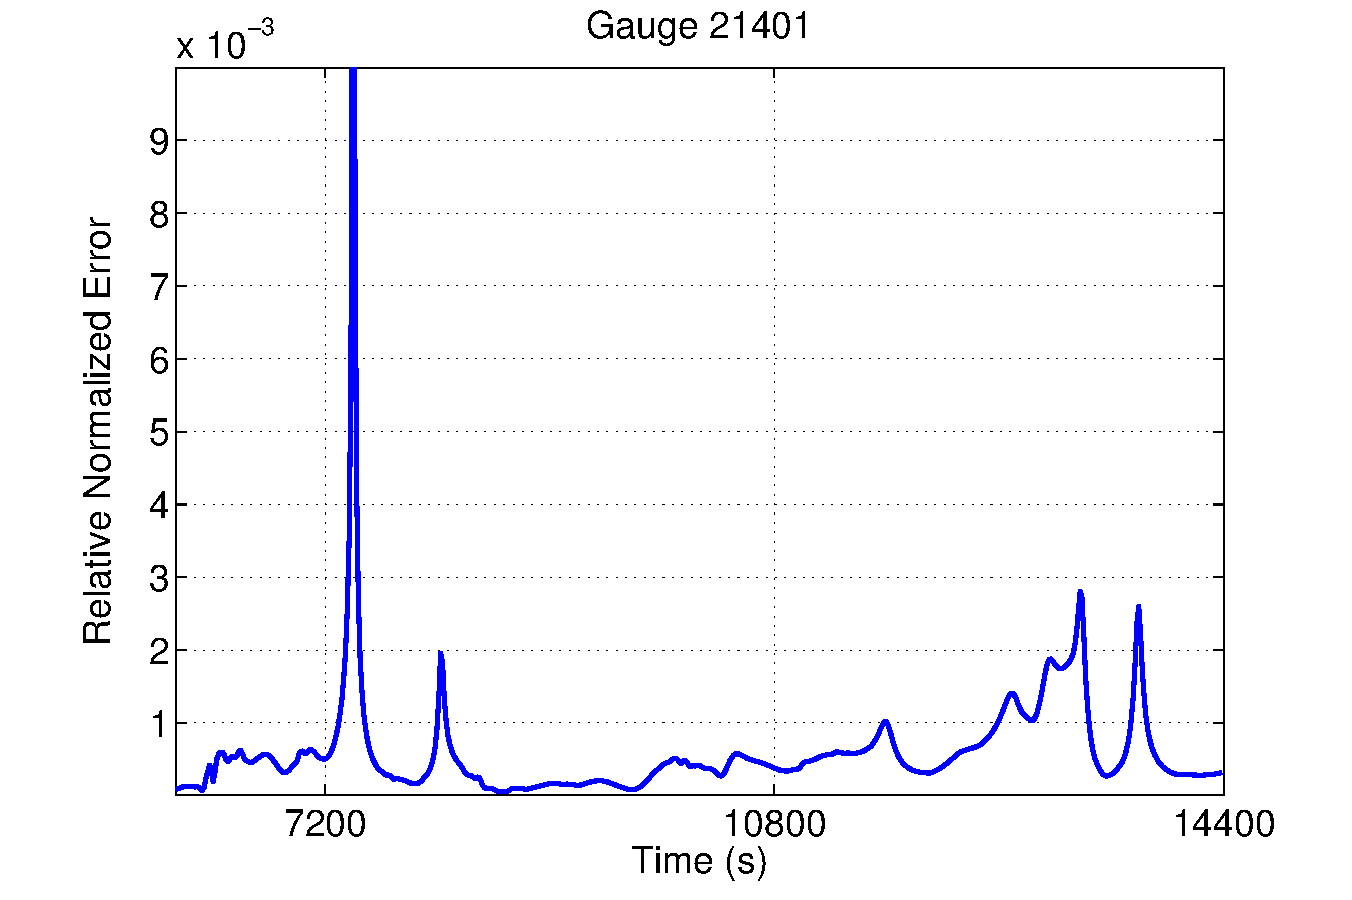
\includegraphics[width=0.5\textwidth]{../figures/error_gauge1.pdf} &
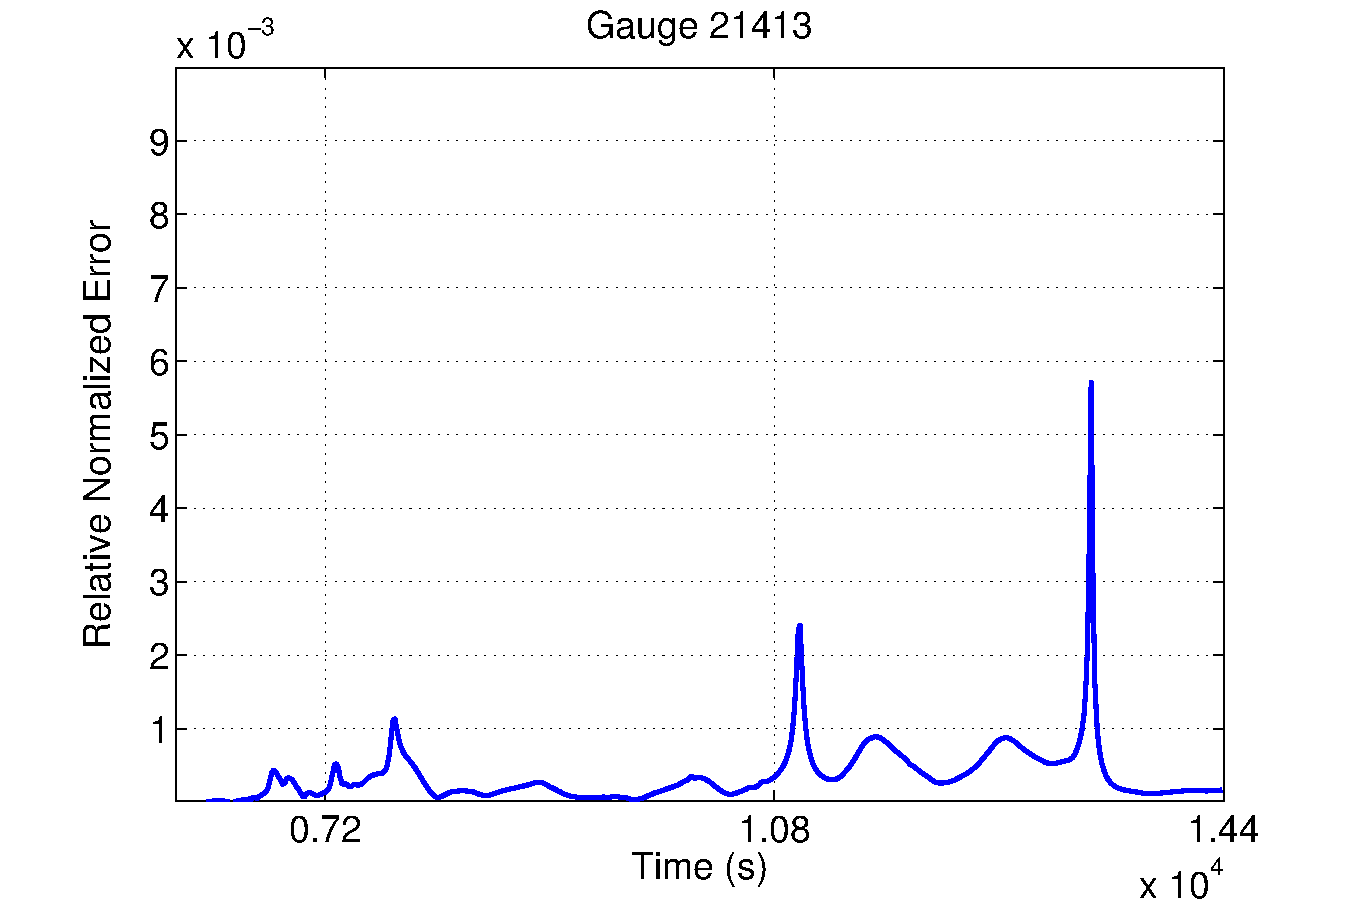
\includegraphics[width=0.5\textwidth]{../figures/error_gauge2.pdf} \\
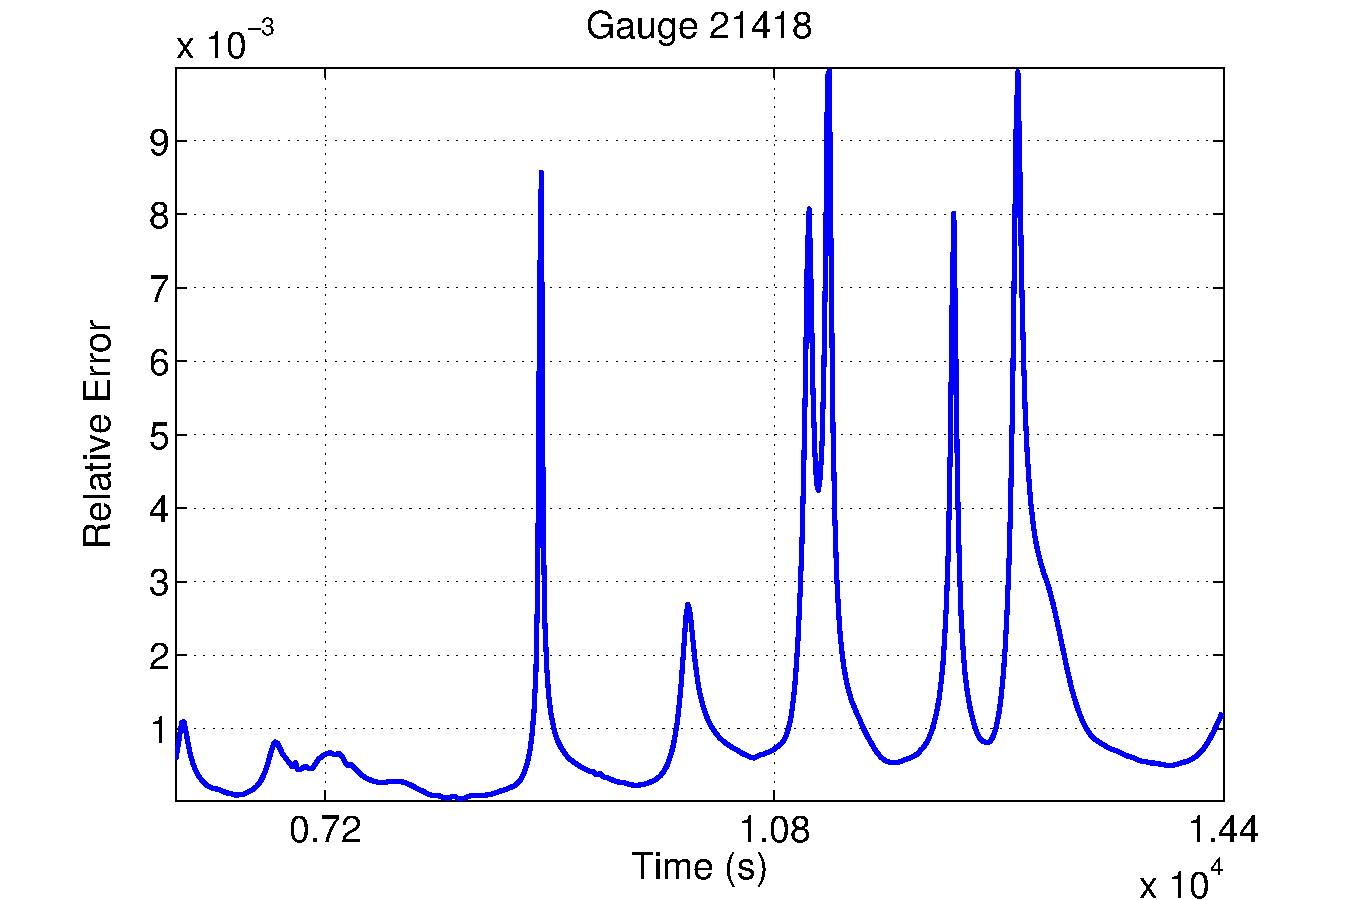
\includegraphics[width=0.5\textwidth]{../figures/error_gauge3.pdf} &
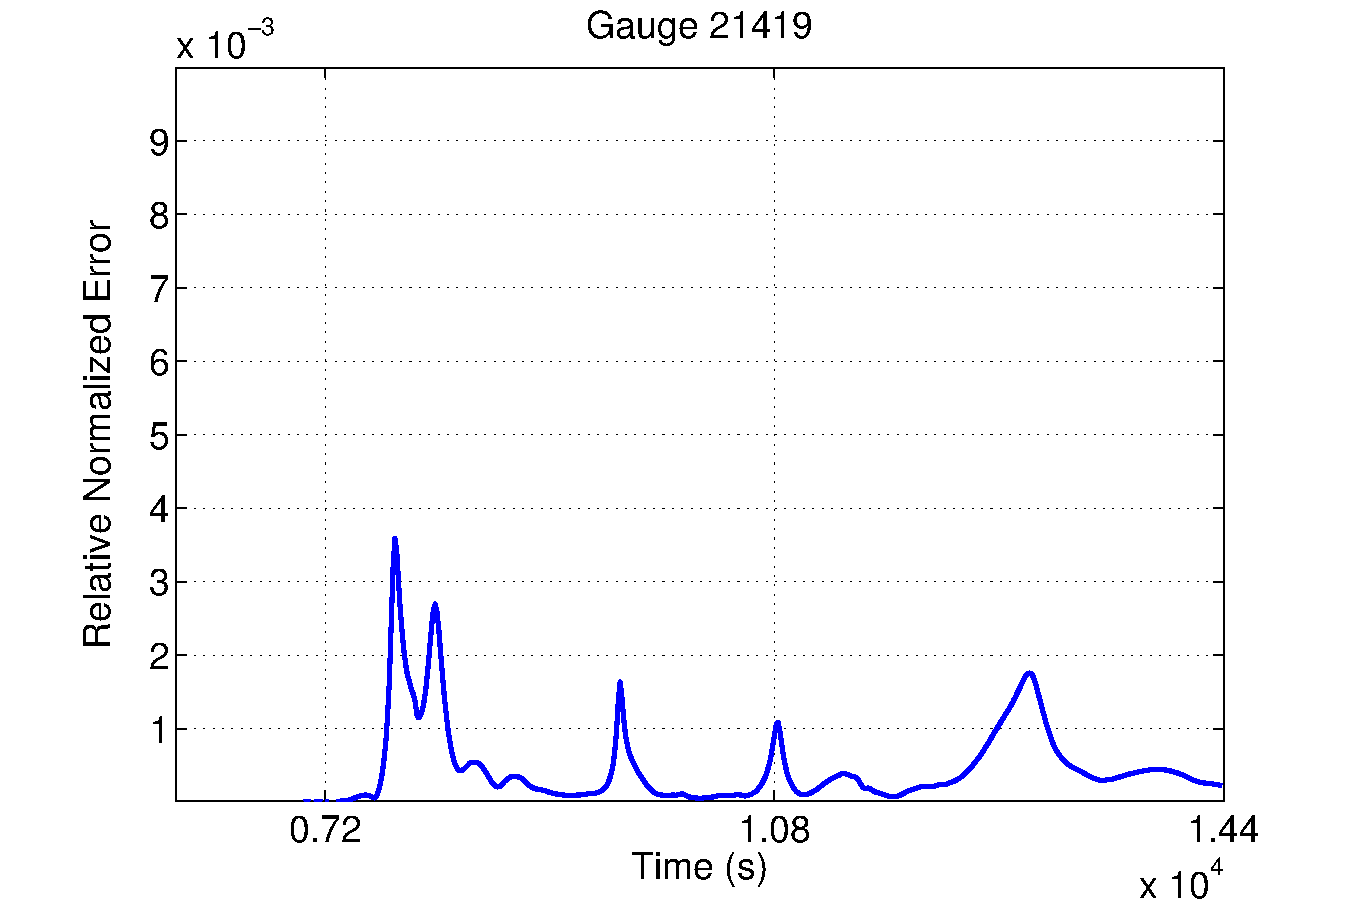
\includegraphics[width=0.5\textwidth]{../figures/error_gauge4.pdf} 

\end{tabular}
\caption{125 Geoclaw realizations at different gauge locations.}
\label{fig:error}
\end{figure}

%Contour maps of the relative normalized error for the entire simulation region are 
%shown in Figure~\ref{fig:error2D} for various depths and dates to confirm the error trends of the
%analysis box.  The error is largest after the wind
%intensifies (bottom row) for all depths. For either day, the maximum
%error is located at 50~m which coincides with the depth of the
%original mixed layer measured by the AXBT. The maximum magnitude
%recorded is about 1\% and occurs on Sep~18. The
%elevated error region is located to the right of the storm and
%extends from the surface down to 50~m, after which the impact of the
%input uncertainty decreases substantially.  For the purpose of our
%current study, and given that the majority of AXBT data are at
%depth, the surrogate's errors are considered acceptable and small.

 
A final check consists of verifying whether the probability density
functions (pdfs) of water surface elevation at the different gauge locations
converges with increased order of the PC representation.  Sample
water surface elevation pdfs are shown in Figure~\ref{fig:pdfs2}
and Figure~\ref{fig:pdfs3}

\begin{figure}[h]
\centering

\begin{tabular}{clcl}
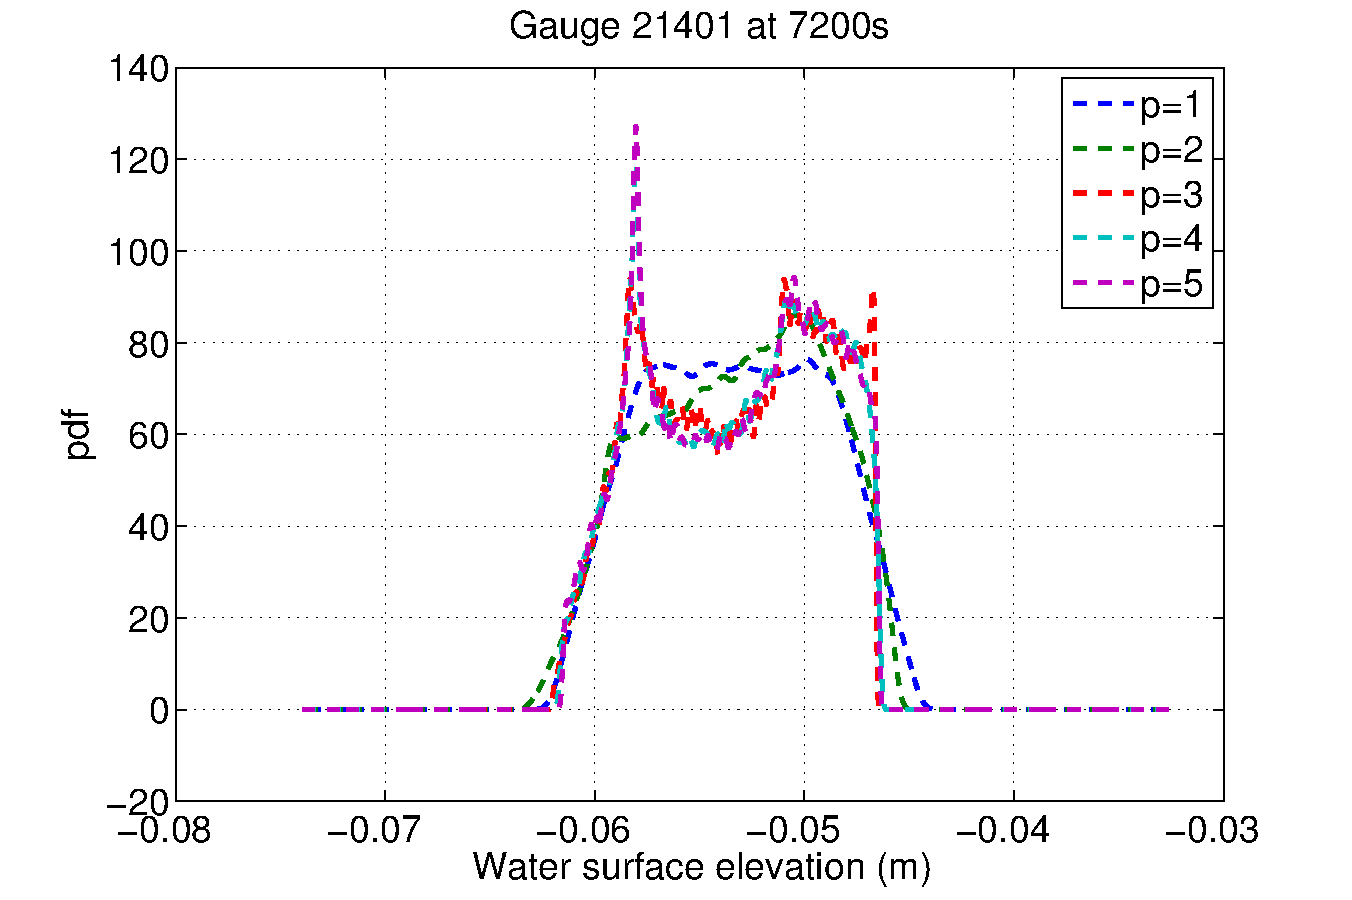
\includegraphics[width=0.5\textwidth]{../figures/pdfs1_2.pdf} &
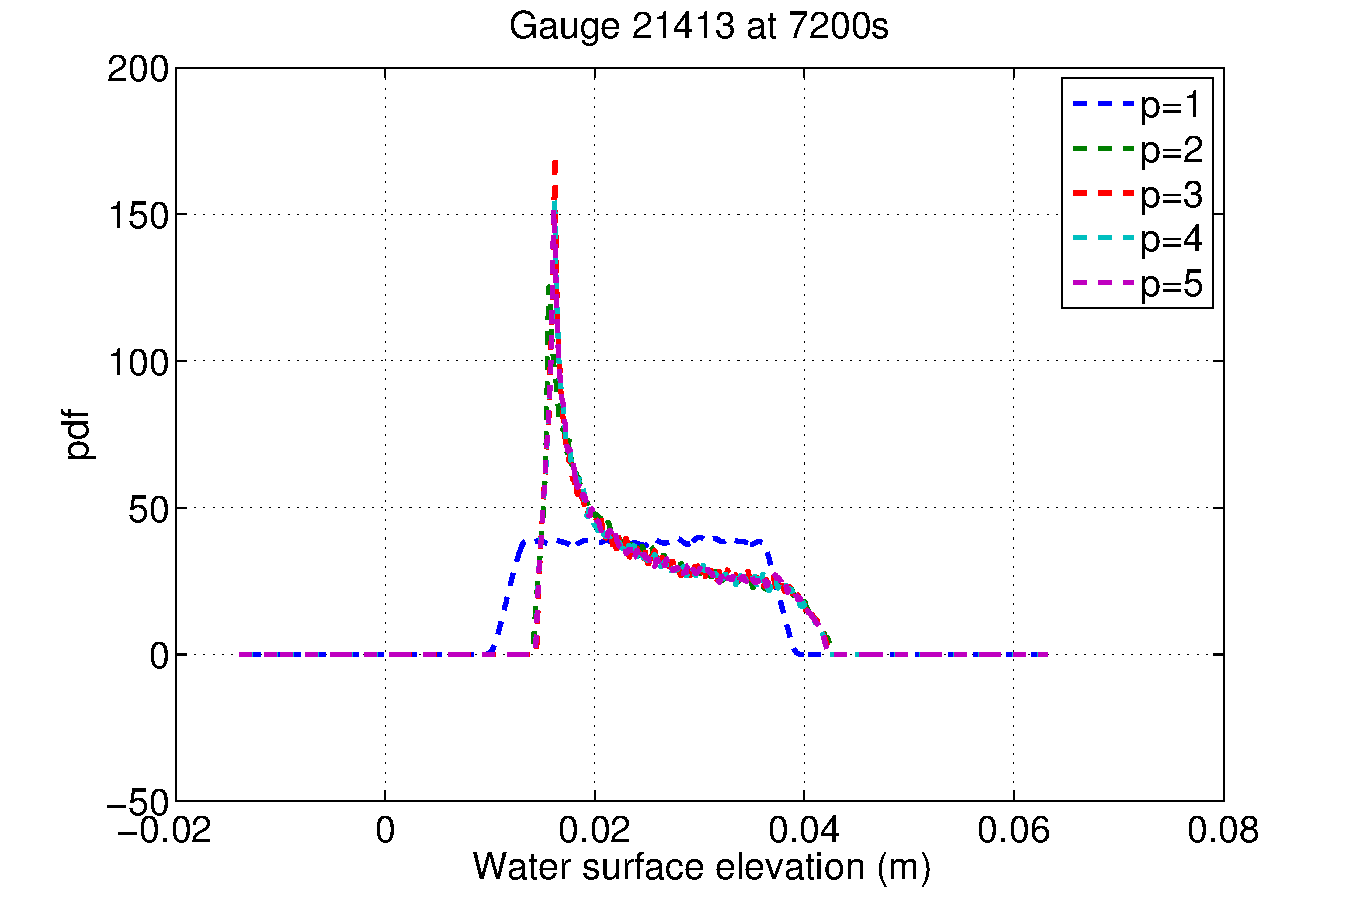
\includegraphics[width=0.5\textwidth]{../figures/pdfs2_2.pdf} \\
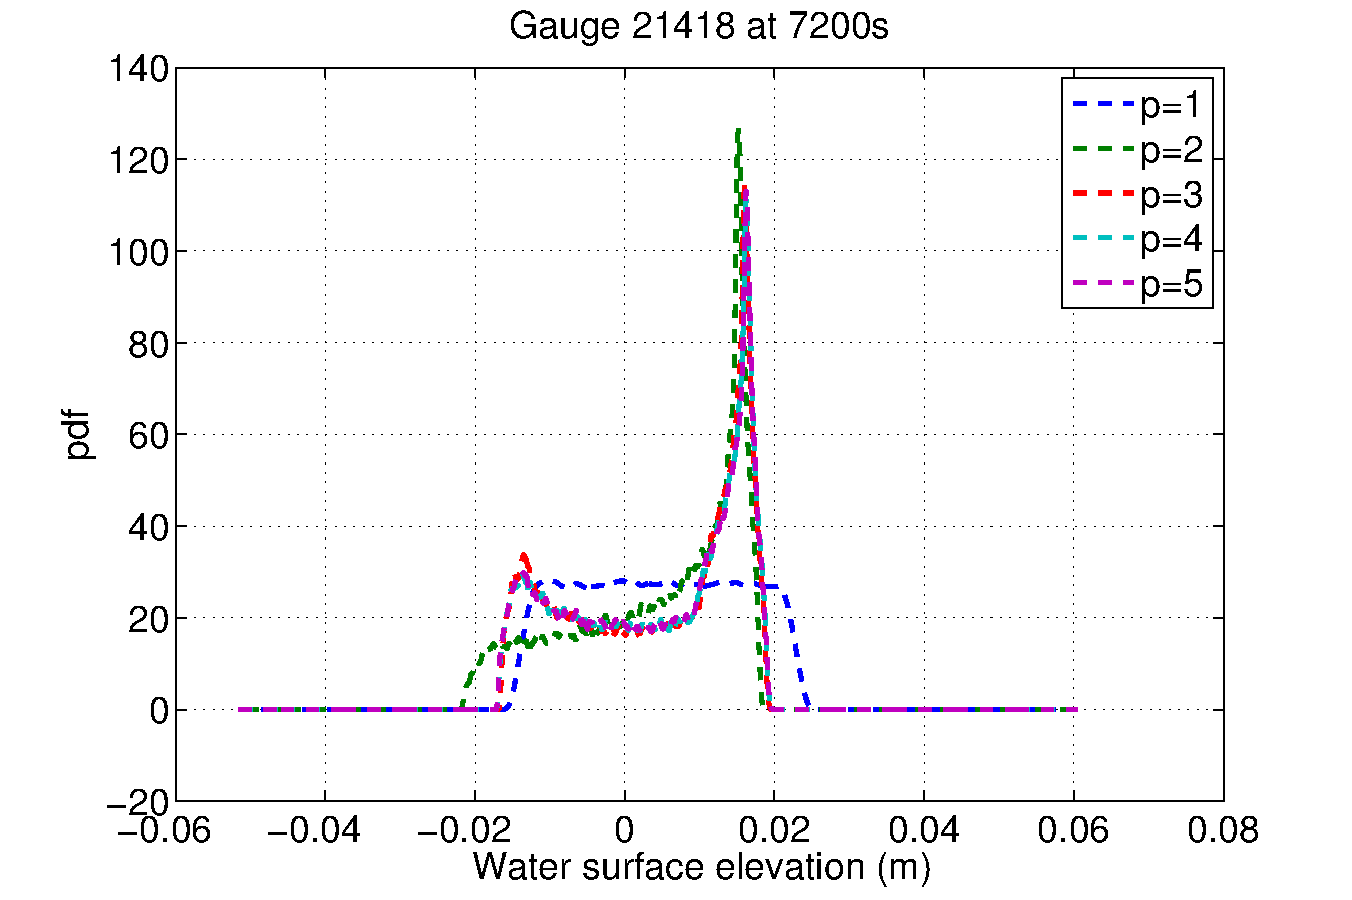
\includegraphics[width=0.5\textwidth]{../figures/pdfs3_2.pdf} &
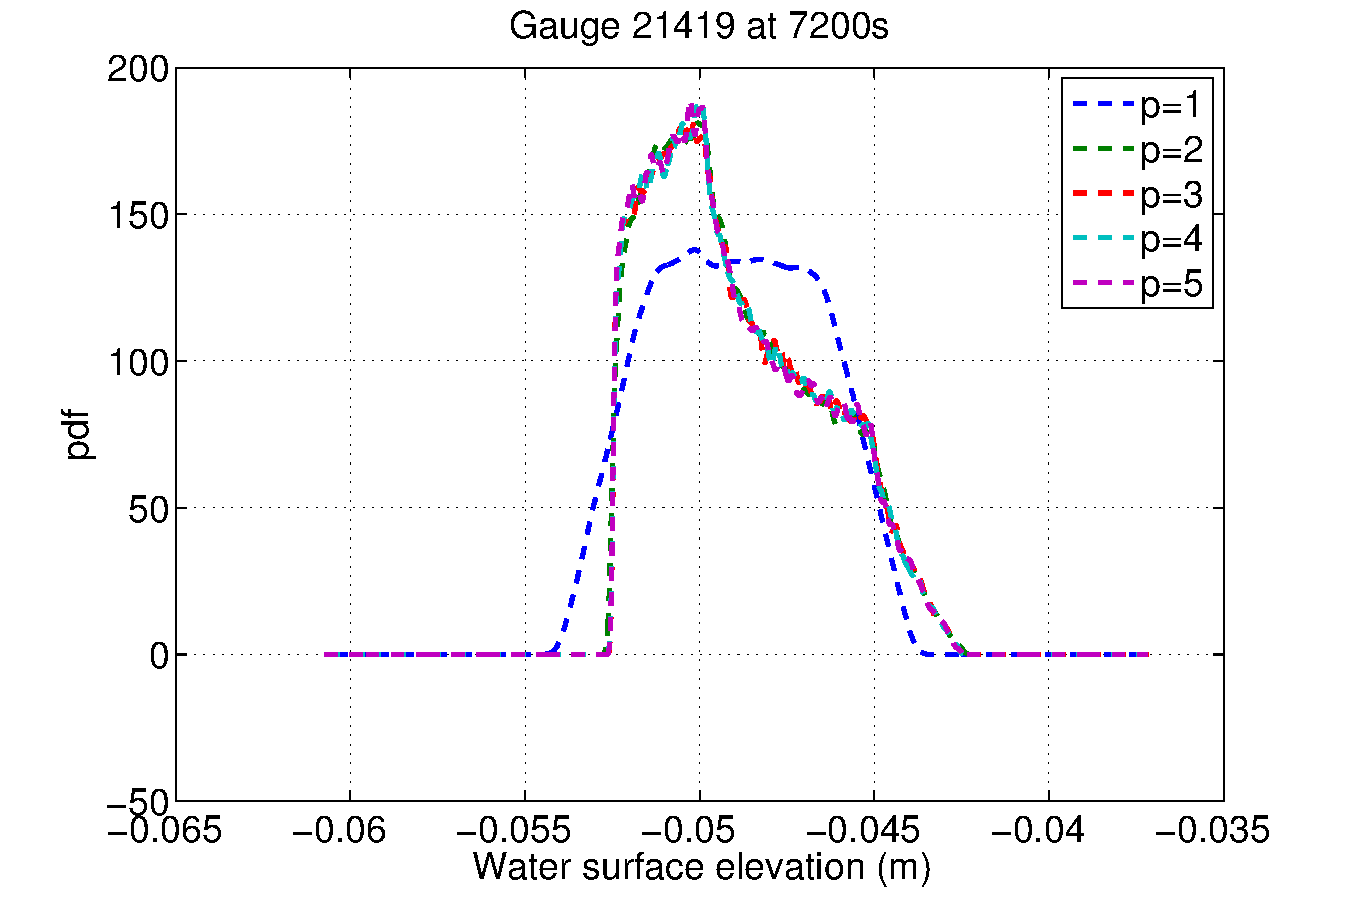
\includegraphics[width=0.5\textwidth]{../figures/pdfs4_2.pdf}
\end{tabular}
\caption{pdf of water surface elevation at the different gauge locations at t = 7200 s.}
\label{fig:pdfs2}
\end{figure}
        
\begin{figure}[h]
\centering
\begin{tabular}{clc}
        
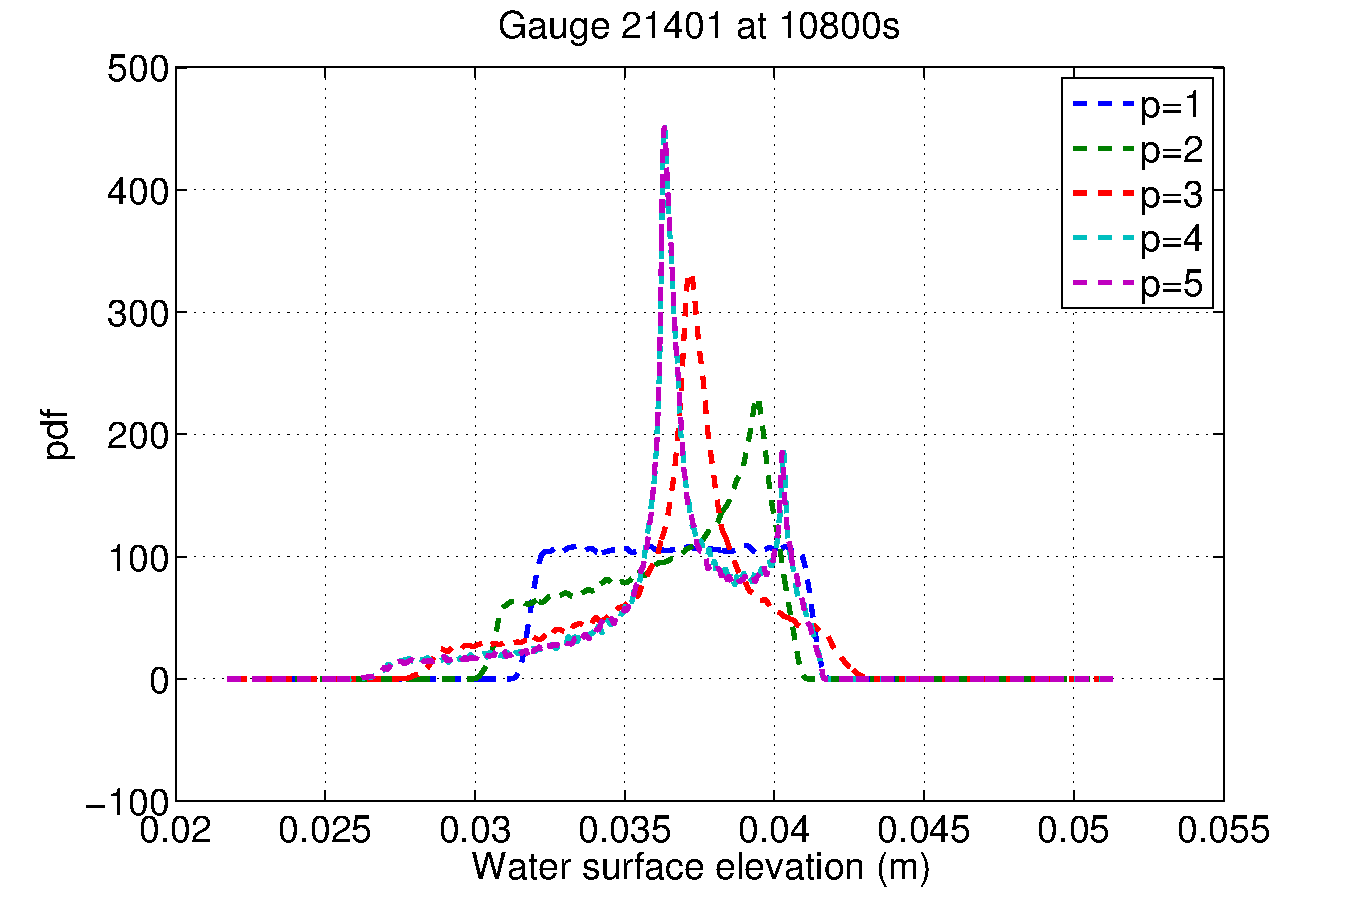
\includegraphics[width=0.5\textwidth]{../figures/pdfs1_3.pdf} &
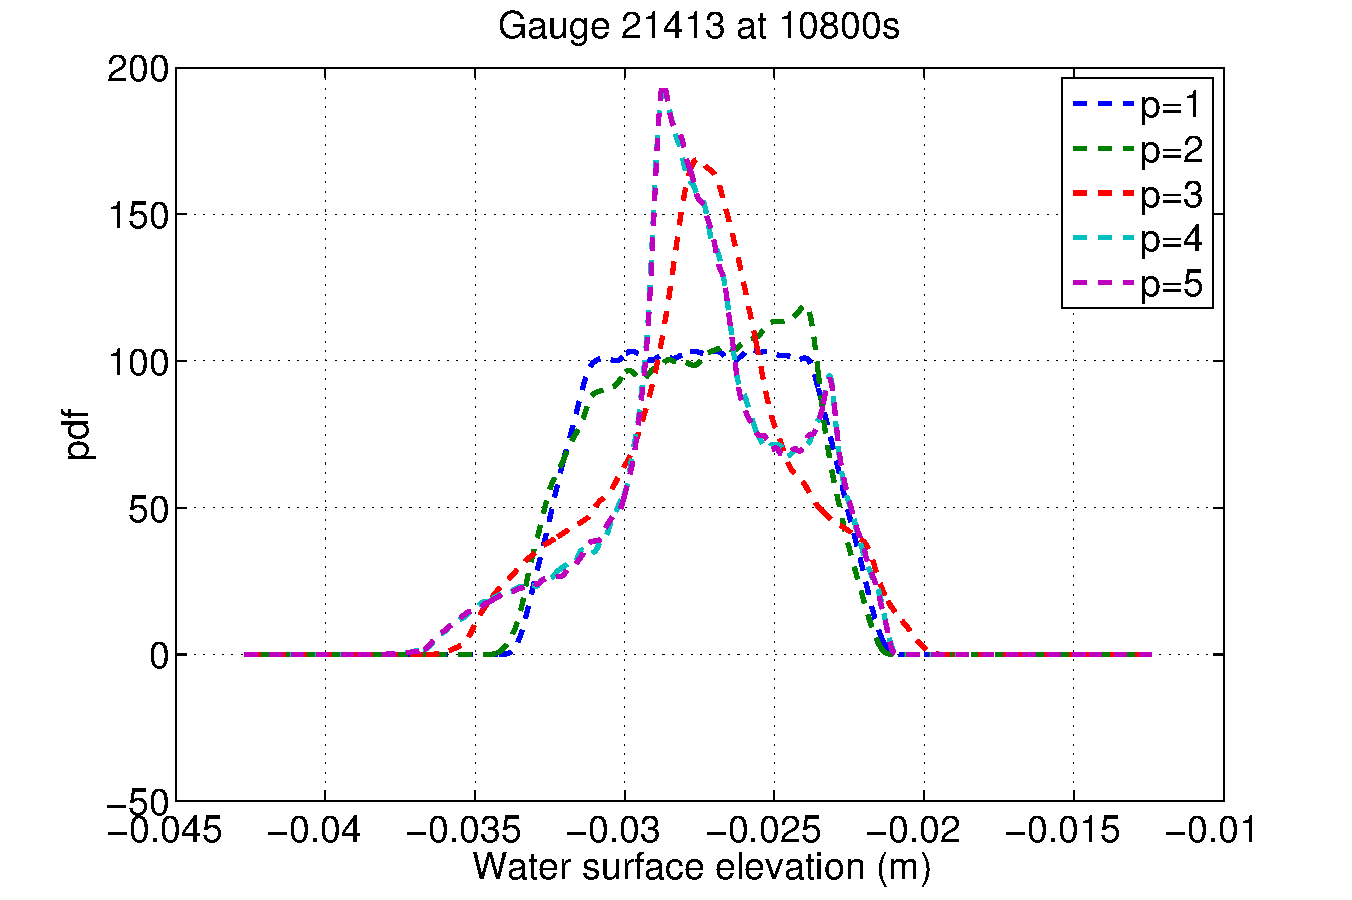
\includegraphics[width=0.5\textwidth]{../figures/pdfs2_3.pdf} \\
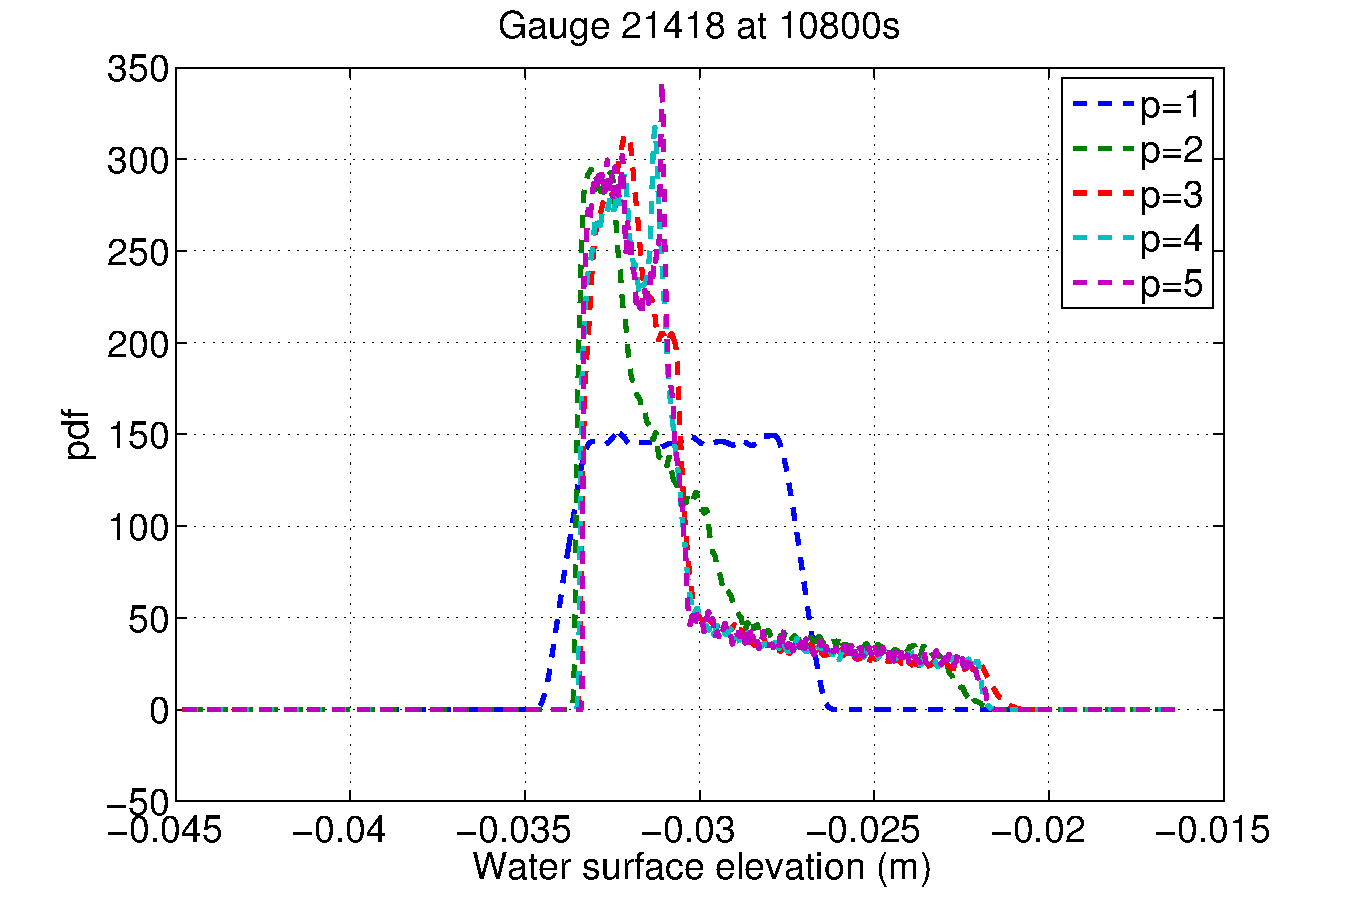
\includegraphics[width=0.5\textwidth]{../figures/pdfs3_3.pdf} &
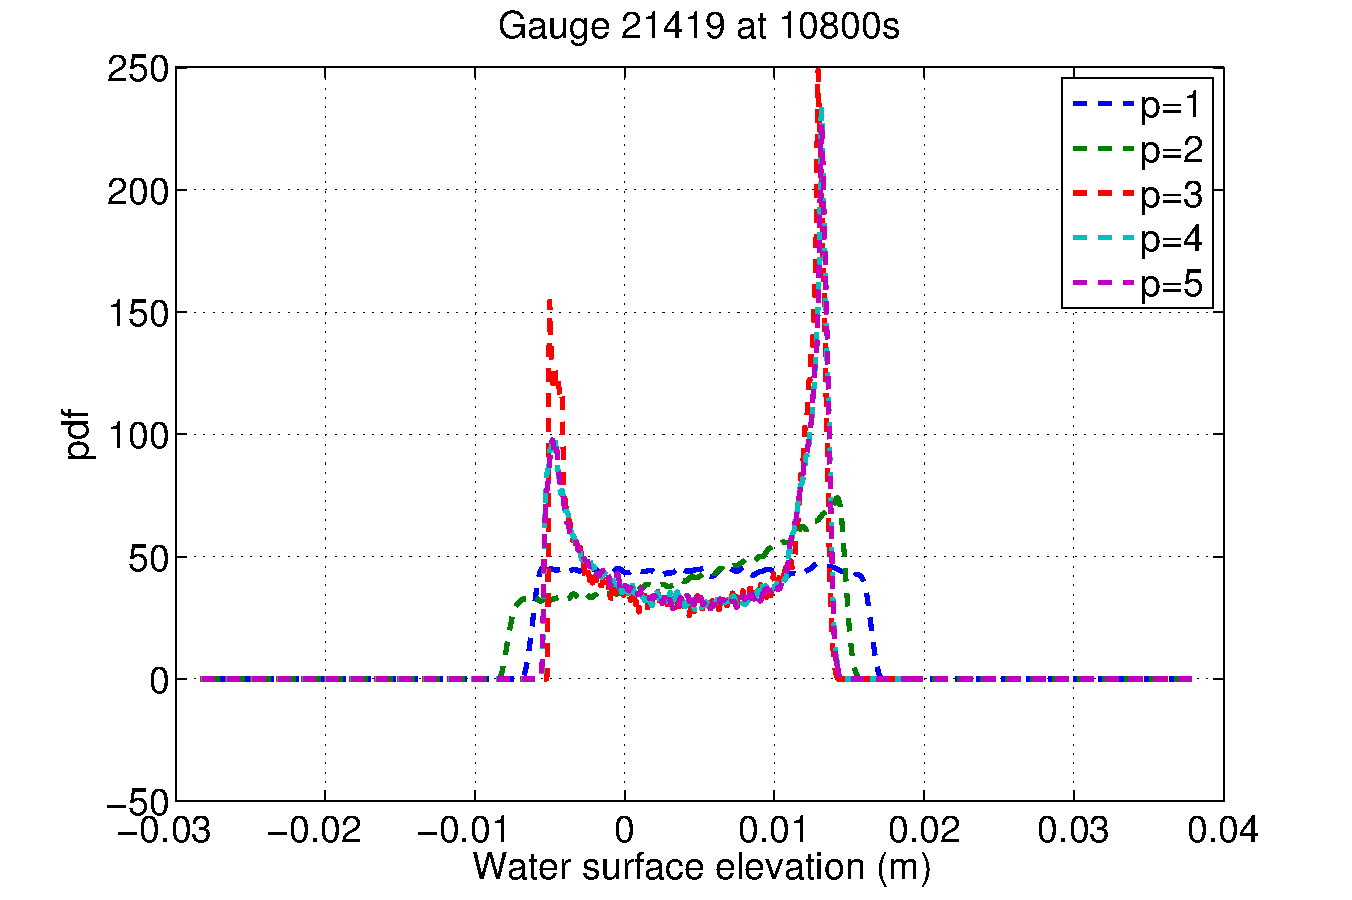
\includegraphics[width=0.5\textwidth]{../figures/pdfs4_3.pdf}
\end{tabular}
\caption{pdf of water surface elevation at the different gauge locations at t = 10800 s.}
\label{fig:pdfs3}
\end{figure}
The different curves
correspond to increased order of PC, from 1 to 5; 
The plots indicate that the double peaked distributions are
well-resolved with order  4 but becomes weakly insenstive to further refinement 
as shown with order 5.

The various error metrics presented above 
provide confidence that the PC expansion is a faithful 
model surrogate. 

\clearpage

